\section{Projection mapping}

FF.


\subsection{Projector modeling}

Over the years, several projection technologies were developed according to the requirements of color fidelity / saturation, image sharpness, brightness, contrast, refresh rate and price. Currently, the video projection market is split between reflective \gls{dlp} and transmissive \gls{lcd} projection technology, with a small percentage of projectors consisting of a hybrid between the two technologies (\gls{lcos}).

For video projection mapping purposes \cite{Raskar1998,Bimber2005,Tan2013,Fujimoto2014}, reflective projectors are better suited than the remaining technologies given their ability to create images with smaller gaps between the projected pixels (smoother images) and they also have higher contrast, better color accuracy / uniformity, much fewer dead pixels and the image quality does not degrade over time. The main stages of the image creation in a \gls{dlp} projector are show in \cref{fig:dlp-projector-diagram-dmd}. The first phase is the generation of light from either a lamp or a \gls{led} / laser array, which is later on condensed on a lens in order to pass through a moving color wheel to become one of the 3 primary additive colors (red, green, blue). The colored light then passes through a shaping lens and hits a \gls{dmd} which has an electronic controllable mirror for each projection pixel that either reflects the light into the projection lens or into a heat sink. Color shading is achieved by controlling how long and how often the micro mirrors in the \gls{dmd} are reflecting each light color into the lens (or into the heat sink).


\begin{figure}[H]
	\begin{floatrow}[2]
		\ffigbox[\FBwidth]
		{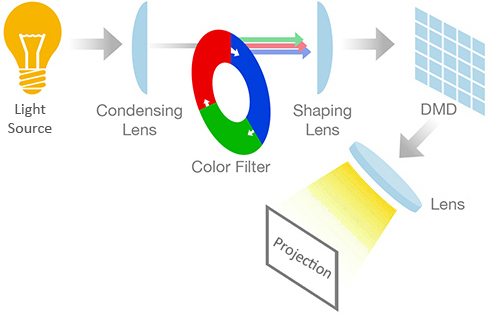
\includegraphics[height=.19\textheight]{dlp-projector-diagram-dmd}}
		{\caption[Single chip \glsentrytext{dlp} diagram]{Single chip \glsentrytext{dlp} diagram\protect\footnotemark}\label{fig:dlp-projector-diagram-dmd}}
		\ffigbox[\FBwidth]
		{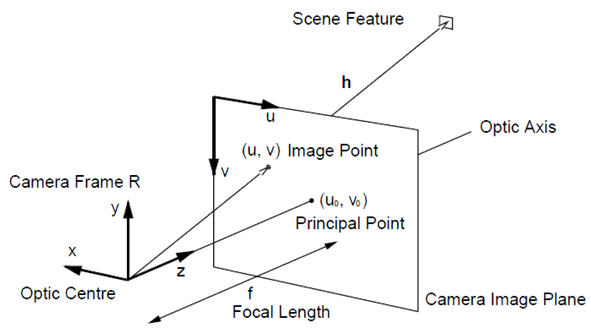
\includegraphics[height=.19\textheight]{camera-intrinsics}}
		{\caption[Pinhole camera model]{Pinhole camera model\protect\footnotemark}\label{fig:camera-intrinsics}}
	\end{floatrow}
\end{figure}
\footnotetext[\the\numexpr\value{footnote}-1\relax]{\url{https://vimeo.com/blog/post/display-tech-home-projectors}}
\footnotetext[\value{footnote}]{\url{http://perso.ensta-paristech.fr/~filliat/Courses/2011_projets_C10-2/BRUNEAU_DUBRAY_MURGUET/monoSLAM_bruneau_dubray_murguet_en.html}}


The mathematical modeling of a \gls{dlp} projector can be seen as an inverse pinhole camera \cite{Hartley2003} (shown in \cref{fig:camera-intrinsics}), given the grid disposition of the mirrors in the \gls{dmd} and the very low distortion that modern \gls{dlp} projectors have. As such, scene rendering can be performed efficiently using the \gls{opengl} projection matrix (shown in \cref{eq:projection-matrix,eq:ndc-matrix,eq:perspective-matrix}), which incorporates the focal lengths (Fx, Fy), principal point (Cx, Cy) and axis skew (S) intrinsic camera parameters (in pixel units). The correction of lens distortion for \gls{dlp} projectors typically uses 3 coefficients for removing radial distortions and 2 coefficients for accounting for the tangential distortions.

{
	\small
	\begin{equation}\label{eq:projection-matrix}
	ProjectionMatrix = \glsentrytext{ndc}Matrix \times PerspectiveMatrix
	\end{equation}
	
	\begin{equation}\label{eq:ndc-matrix}
	NDCMatrix = 
	\begin{bmatrix}
	\frac{2}{ImageWidth} & 0 & 0 & -1 \\
	0 & \frac{2}{ImageHeight} & 0 & -1 \\
	0 & 0 & \frac{-2}{ClipFar - ClipNear} & \frac{-(ClipFar + ClipNear)}{ClipFar - ClipNear} \\
	0 & 0 & 0 & 1
	\end{bmatrix}
	\end{equation}
	
	
	\begin{equation}\label{eq:perspective-matrix}
	PerspectiveMatrix = 
	\begin{bmatrix}
	Fx & S & -Cx & 0 \\
	0 & Fy & -Cy & 0 \\
	0 & 0 & ClipNear + ClipFar & ClipNear \times ClipFar \\
	0 & 0 & -1 & 0
	\end{bmatrix}
	\end{equation}
}


\subsection{Projector calibration}

High accuracy projection mapping requires proper hardware / software calibration of the camera / projector and also appropriate positioning within the intended workspace in order to avoid occlusions caused by the objects 3D shape or the human operators. This calibration aims to compute the intrinsic parameters of the projector (that do not change when the projector is moved within the workspace) along with the extrinsic parameters that are needed to know where is the projector in the global reference frame in order to be able to do proper 3D rendering of the scene that will be projected.

The intrinsic parameters of a \gls{dlp} projector can be computed using image analysis of complementary gray code patterns (example in \cref{fig:dlp-calibration-pattern-wall}) projected into a chessboard. The calibration system proposed in \cite{Moreno2012} was used to retrieve the 5 intrinsic parameters (Fx, Fy, Cx, Cy, S) of the projector along with the 3D position and rotation of the projector in relation to the camera (that remains firmly attached to the projector support for fast recalibration of the extrinsic parameters). It was used 5 sets of 42 gray code image patterns captured with the chessboard in different positions and orientations in relation to the projector, that was pointing to the table workspace at a distance of 0.81 meters. After calibration it was projected a validation pattern to evaluate the accuracy of the projection, and as can be seen in \cref{fig:dlp-projected-chessboard}, the white squares were projected into the chessboard with sub-millimeter accuracy.

\begin{figure}[H]
	\begin{floatrow}[2]
		\ffigbox[\FBwidth]
		{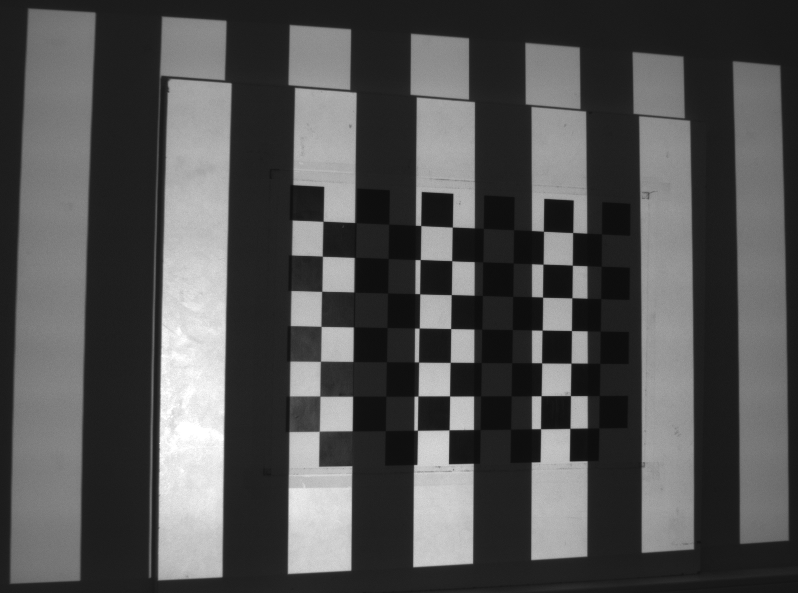
\includegraphics[height=.205\textheight]{dlp-calibration-pattern-wall}}
		{\caption{One of the \glsentrytext{dlp} projector calibration patterns}\label{fig:dlp-calibration-pattern-wall}}
		\ffigbox[\FBwidth]
		{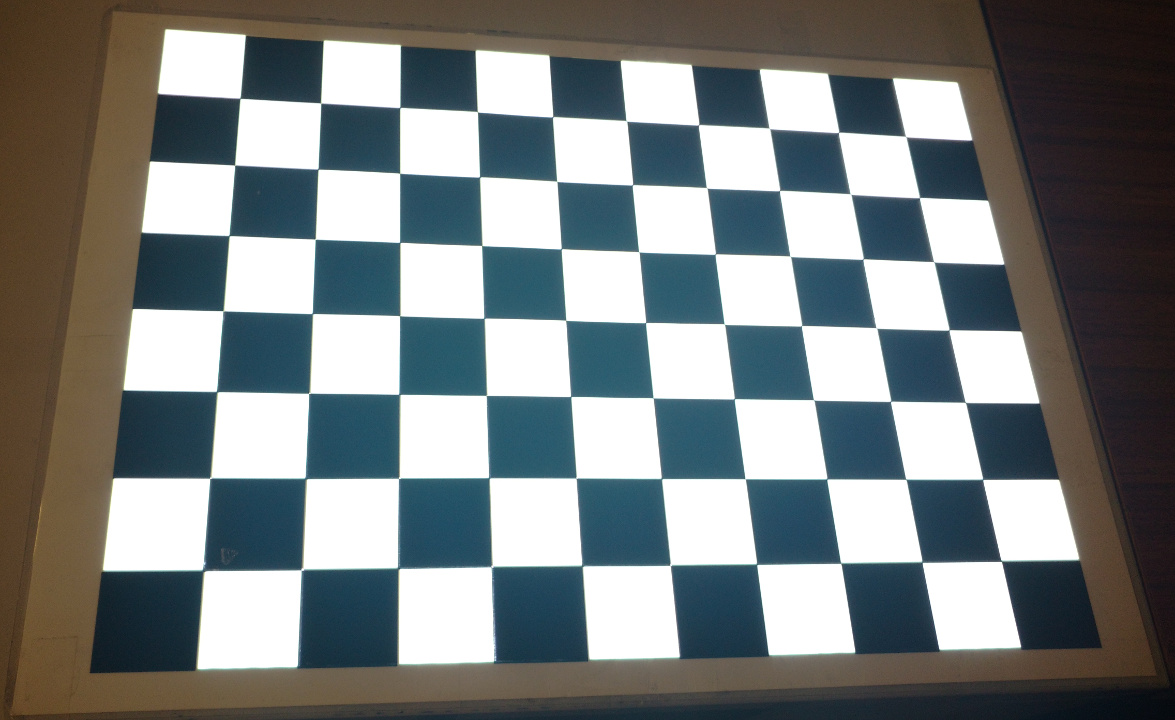
\includegraphics[height=.205\textheight]{chessboard}}
		{\caption{\glsentrytext{dlp} projector validation pattern}\label{fig:dlp-projected-chessboard}}
	\end{floatrow}
\end{figure}

After having the intrinsic parameters of the camera and projector along with the relative position of the projector in relation to the camera, computing the global position of the projector in relation to the chessboard reference frame can be done by multiplying the $4 \times 4$ homogeneous matrix that gives the transformation from the chessboard bottom left corner (shown in \cref{fig:chess-board-detection}) to the camera, with the $4 \times 4$ homogeneous matrix that gives the transformation from the camera to the projector.

\begin{figure}[H]
	\centering
	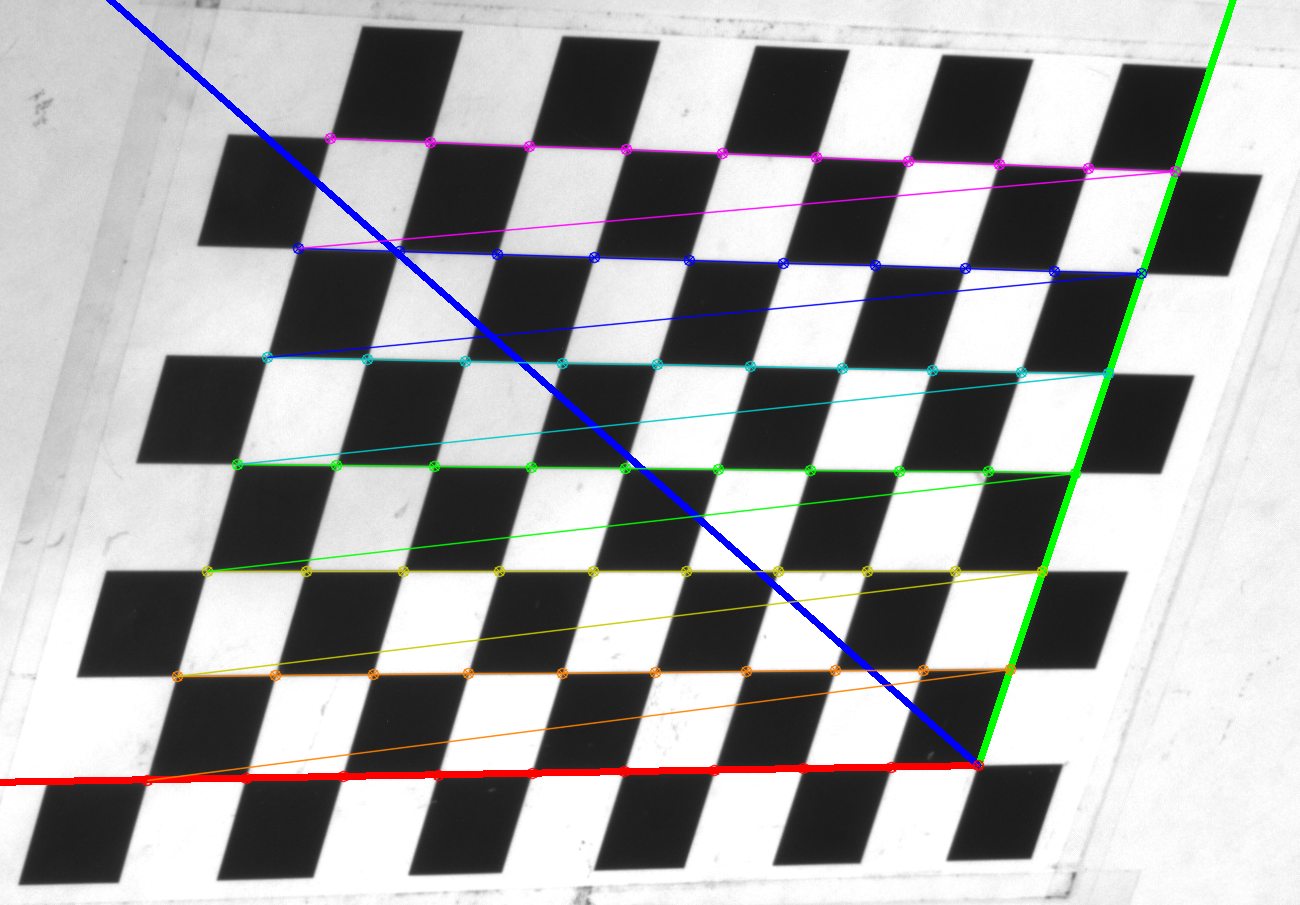
\includegraphics[width=0.47\linewidth]{chess-board-detection}
	\caption{Example of chessboard origin detection}
	\label{fig:chess-board-detection}
\end{figure}


\subsection{Scene rendering}

For achieving accurate projection mapping, the Gazebo simulator camera implementation was improved to allow the setting of a custom projection matrix in order to perform 3D rendering with a camera model that simulates the projector intrinsic parameters. Moreover, it was added the possibility to dynamically change image, video and text during runtime, for allowing the display of the relevant information for each assembly step.
For efficient 3D scene rendering, the Gazebo simulator relies on the cross platform open source Ogre3D graphics engine\footnote{\url{http://www.ogre3d.org}}, that in turn uses the \gls{opengl} \gls{gpu} \glspl{api} to take advantage of the massively parallel graphics cards currently available to generate raster images for the \gls{dlp} projector (example in \cref{fig:scene-rendering}).

For user interface, the Gazebo simulator allows visual inspection of the scene while also giving the option to add new objects or move and rotate existing models. Moreover, for lightweight rendering, it can also start in server mode without a \gls{gui}.

\begin{figure}
	\centering
	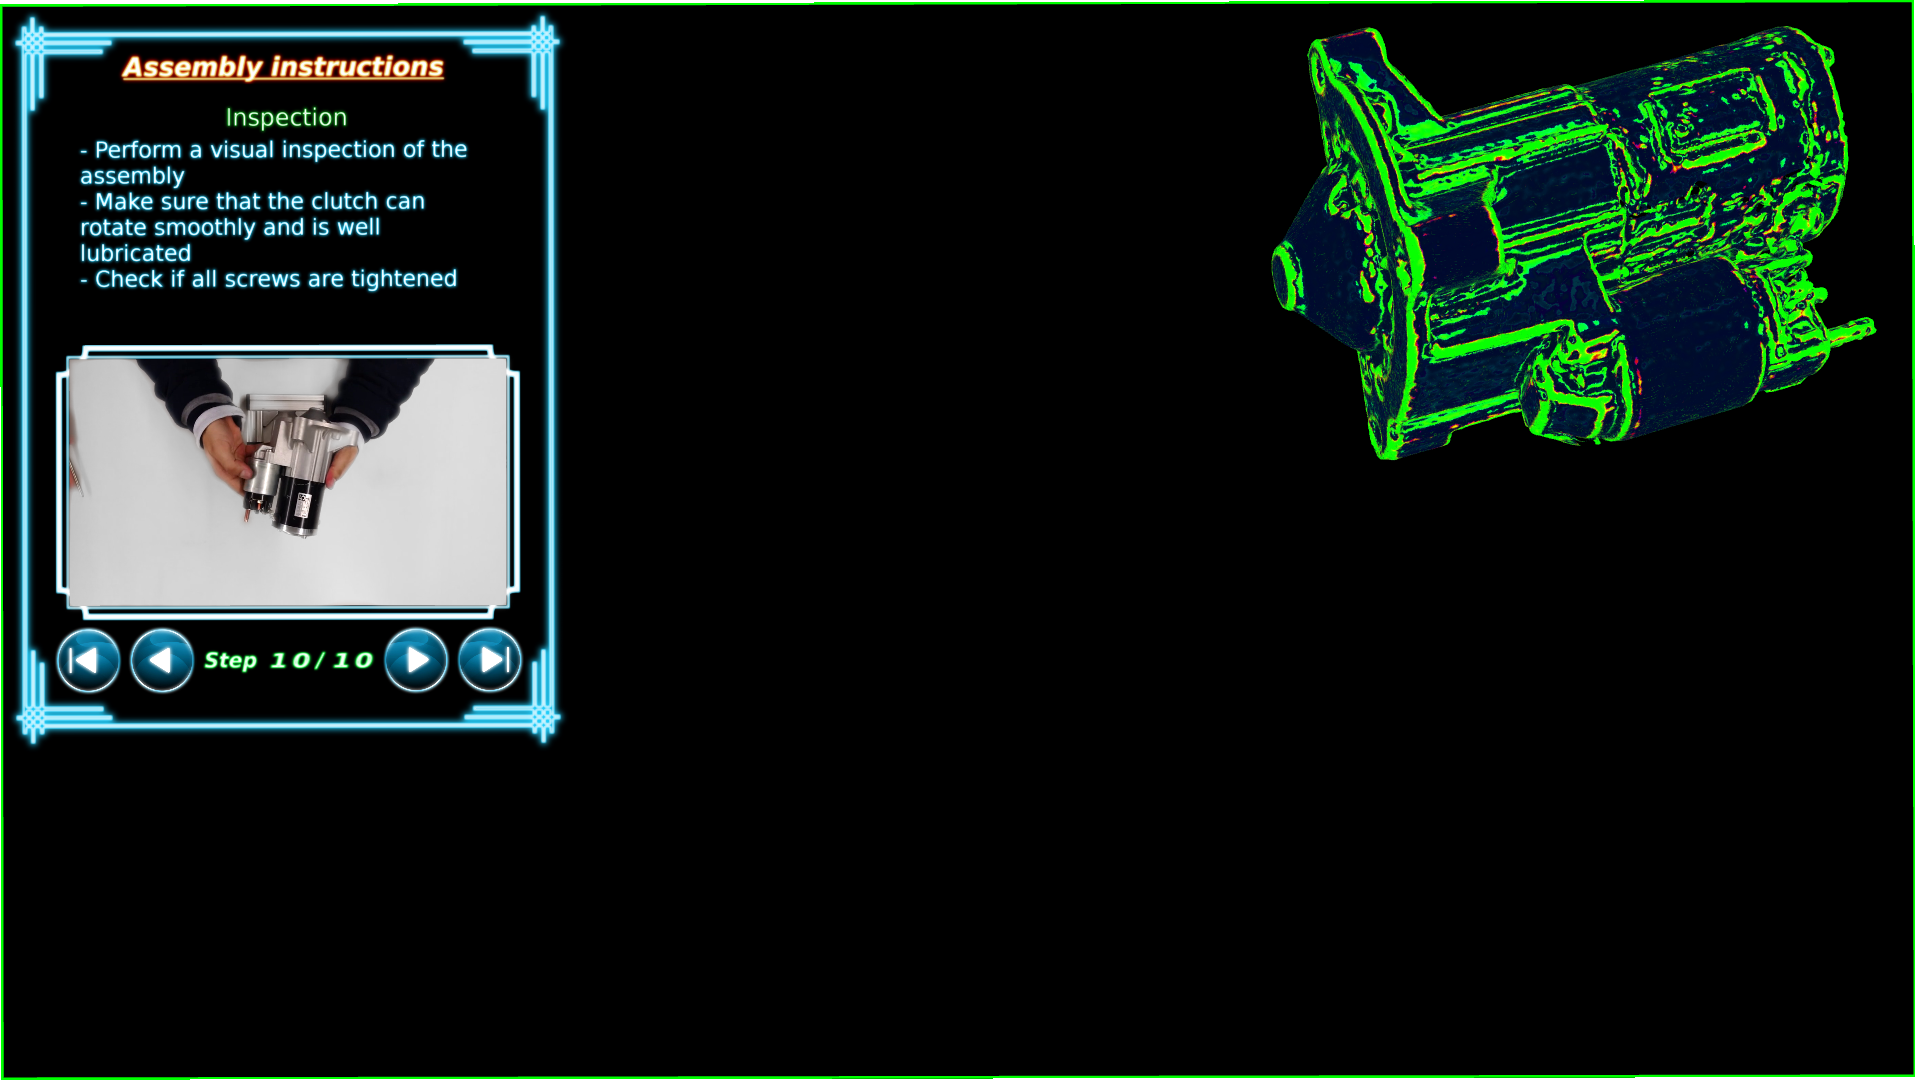
\includegraphics[width=0.77\linewidth]{scene-rendering}
	\caption{3D scene rendering using the Gazebo simulator}
	\label{fig:scene-rendering}
\end{figure}



\section{Human machine interaction}

\begin{itemize}
	\item Modeling of the user interaction with the projected interface by defining a set of Regions of Interest (ROIs) in which the 3D sensor data falls
	\item When a minimum number of points falls within a given ROI, the points centroid is extracted and:
	\begin{itemize}
		\item If it is a button, the user needs to hold the finger for 0.2 seconds to trigger the action. Moreover, to avoid unintentional triggering , the user needs to remove the finger from the ROI to trigger the action again
		\item If it is the video seek bar, the video position is computed considering the height of the video and the relative position of the finger in relation to the button of the video
	\end{itemize}
\end{itemize}

\textbf{Supported actions}
\begin{itemize}
	\item Go to the first assembly step
	\item Go to the previous assembly step
	\item Go to the next assembly step
	\item Go to the last assembly step
	\item Pause the video
	\item Change the position of the video (seek)
\end{itemize}

\begin{figure}[H]
	\begin{floatrow}[2]
		\ffigbox[\FBwidth]
		{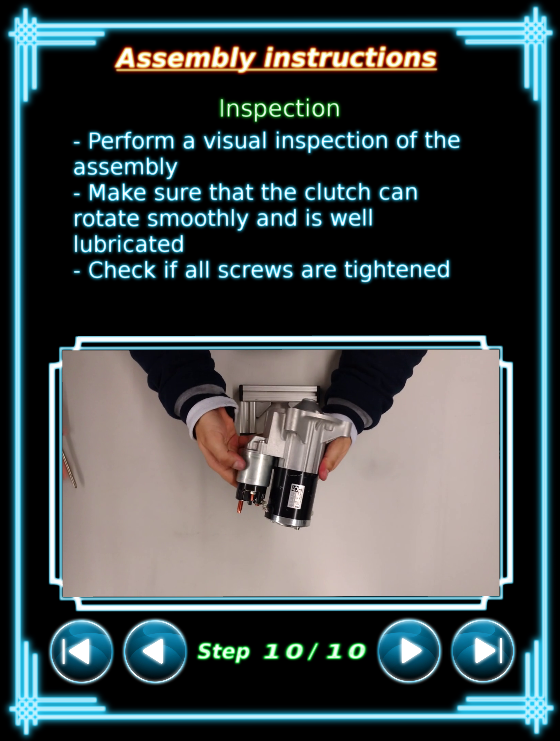
\includegraphics[height=.33\textheight]{human-machine-interface}}
		{\caption{Rendering of the human machine interface}\label{fig:human-machine-interface}}
		\ffigbox[\FBwidth]
		{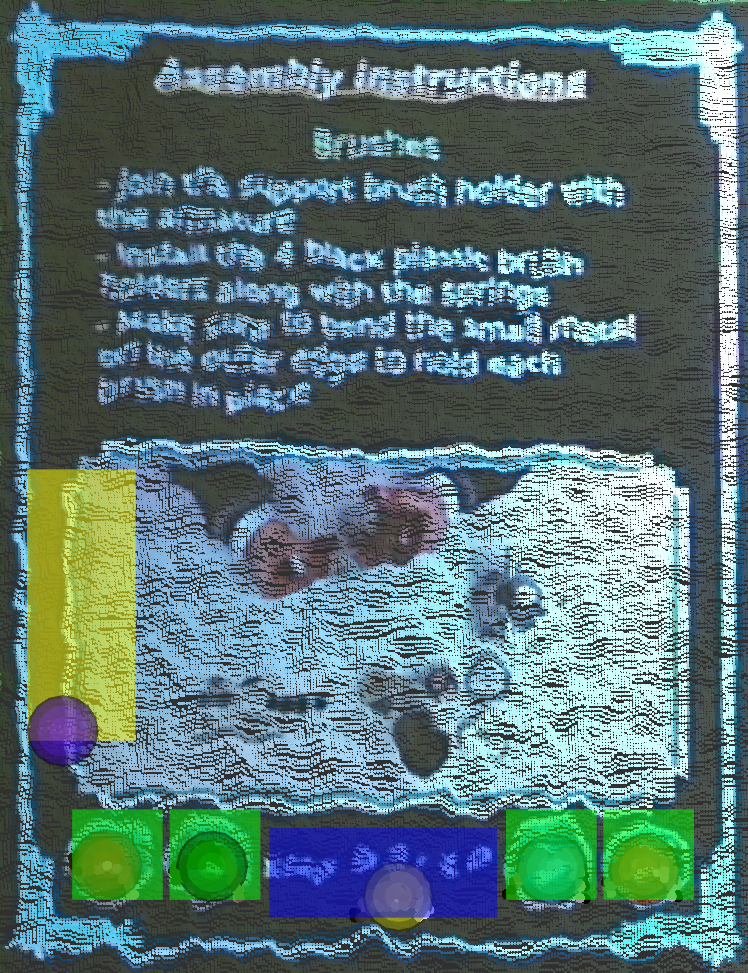
\includegraphics[height=.33\textheight]{interaction-rois}}
		{\caption{Regions of interest for the human machine interaction interface}\label{fig:interaction-rois}}
	\end{floatrow}
\end{figure}


\section{Object 3D reconstruction}

\begin{itemize}
	\item Usage of the David Laser structured light system to obtain the 3d mesh model of the assembled object (no CAD was available)
\end{itemize}

\begin{figure}[ht]
	\centering
	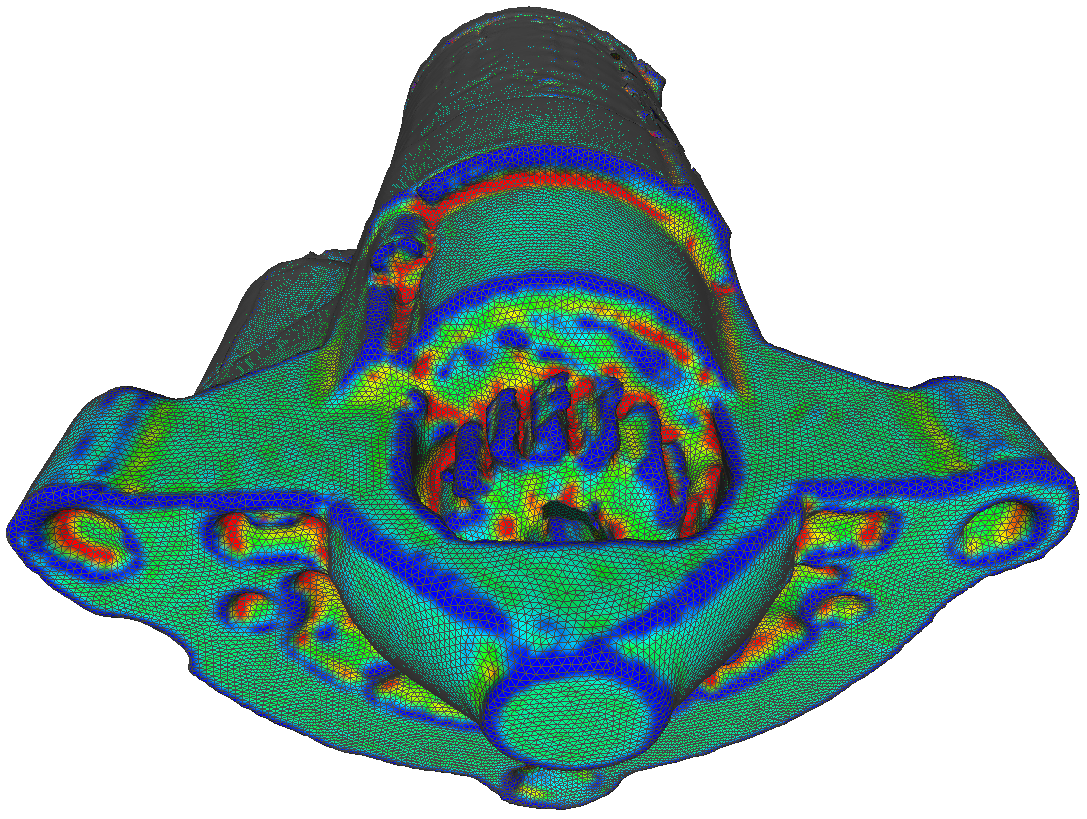
\includegraphics[height=.25\textheight]{object-reconstruction-back}
	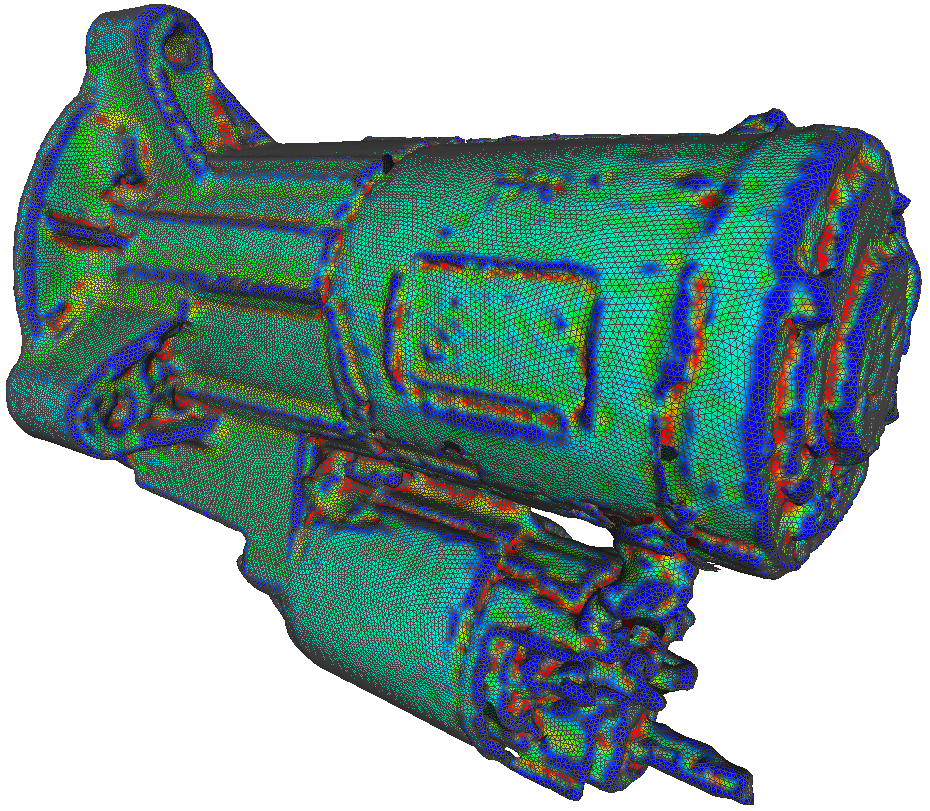
\includegraphics[height=.25\textheight]{object-reconstruction-front}
	\caption{3D model of the starter motor reconstructed using structured light}
\end{figure}


\section{Object recognition}

reference models


\subsection{Point cloud assembly}

The object recognition system can use any sensor that provides point clouds, namely RGB-D / \gls{tof} cameras, \glspl{lidar} and stereo vision systems. Each of these types of sensors have very different operation rates and measurement accuracy. As such, the localization system allows the assembly of several sensor scans using a circular buffer in order to reduce the impact of sensor noise and increase the observed surface area of the objects.


\subsection{Filtering and down sampling}

The time it takes to perform cloud registration increases considerable as the amount of points in the sensor point cloud and in the reference map becomes larger. As such, adjusting the level of detail of the point clouds by using voxel grids gives some control over the desired localization accuracy and the computational resources that will be required. This stage is also useful to mitigate the measurement errors of the depth sensors, since the centroid of a voxel that contains points from several scans will be closer to the real surface (if the voxels have dimensions slightly larger than the expected measurement errors).

The localization system allows the application of several preprocessing algorithms (algorithm type / configuration and execution order customizable). The next sections detail some of these methods that can be used to filter and downsample point clouds.


\subsection{Normal estimation}

Most of feature detection, description and matching algorithms along with some registration methods rely on the point's surface normal and curvature. These algorithms analyze the neighborhood of a given point in order to compute the line / surface normal, and as such, the correct specification of what points should be included in the estimation is crucial to achieve accurate results. This depends on the environment geometry and the level of detail that is required, and is usually done by specifying a radius distance or by limiting the number of neighboring points to use.


\subsection{Keypoint detection}

Aligning two point clouds with overlapping views of the environment requires the establishment of point correspondences. If both point clouds have similar sensor origins, these can be determined with nearest neighbor's searches and filtered with correspondence rejectors (using other point properties such as reflectance and color). But if they were acquired in two very different positions, then more advanced techniques must be employed.

One of those techniques uses histograms to describe the geometric properties of the environment around a given point. This allows points to be matched even if they have completely different Euclidean coordinates. Also, by using histograms and sampling techniques, these descriptors are much more robust against sensor noise and varying level of point density. However, these advantages come with a heavy computational cost, and as such, point descriptors should only be computed on the most descriptive areas of the environment.

Identifying these environment points is known as feature / keypoint detection \cite{Filipe2014}, and usually involves finding interesting points, such as corners and edges. Besides uniqueness, these points must also be repeatable. This means that the detection algorithms should be able to find the same points even if they are present in different point clouds with sensor noise and varying point density. This is of the utmost importance, because if the same keypoints are not identified on both clouds, then matching the point descriptors will likely fail.

Currently, the localization system can use the \gls{sift} \cite{Lowe2004} algorithm on the point's curvature or the \gls{iss3d} \cite{Zhong2009} keypoint detector on the point's normals.


\subsection{Keypoint description}

Describing a keypoint usually involves analyzing its neighboring points and computing a given metric or histogram that quantifies the neighbor's relative distribution, their normals angular relation, associated geometry or other metrics that are deemed useful. Several approaches were suggested over the years according to different recognition needs and they are the basis of feature matching algorithms used in the initial pose estimation.

The localization system can use most of the keypoint descriptors available in \gls{pcl}, namely the \gls{pfh} \cite{Rusu2008a}, the \gls{fpfh} \cite{Rusu2009}, the \gls{shot} \cite{Tombari2011}, the \gls{sc3d} \cite{Frome2004}, the \gls{usc} \cite{Tombari2010} and the \gls{esf} \cite{Wohlkinger2011}.


\subsection{Cloud registration}

Point cloud registration is the process of finding the transformation matrix (usually translation and rotation only) that when applied to a given ambient cloud will minimize an error metric (such as the mean square error of the ambient point cloud in relation to a given reference point cloud). Several approaches were suggested over the years and they can be categorized as point or feature cloud registration.


\subsubsection{Initial alignment with keypoints descriptor matching}\label{subsec:localization-system_feature-registration}

Feature registration is the process of matching keypoint descriptors in order to find an initial alignment between two point clouds. The proposed localization system uses a feature registration method similar to the \gls{sacia} algorithm presented in \cite{Rusu2009}. It uses a \gls{ransac} approach to select the best registration transformation after a given number of iterations. In each iteration a subsample of randomly selected descriptors from the ambient cloud is retrieved. Then for each of these descriptors, $k$ best matching descriptors in the reference point cloud are searched (using a kd-tree) and one of them is chosen randomly (this improves robustness against noise in the sensor data and changes in the environment that are not yet integrated into the map). Later after having filtered these correspondences between ambient and reference descriptors, the registration matrix is computed. If this registration matrix results in a point cloud overlap that has a minimum of inliers percentage (a point in the ambient cloud is an inlier if it has a point in the reference cloud closer than a given distance), then it is considered an acceptable initial pose and is saved (to allow a localization supervisor to analyze the distribution of the acceptable initial poses). In the end of all iterations, the best initial pose (if found) is refined with a point cloud registration algorithm.


\subsubsection{Final alignment with point cloud error minimization}

Point cloud registration algorithms such as \gls{icp} \cite{Besl1992} (with its several known variations \cite{Rusinkiewicz2001,Pomerleau2013} like \gls{icp} point-to-point, \gls{icp} point-to-point non-linear, \gls{icp} point-to-plane and generalized \gls{icp} \cite{Segal2009}) and the \gls{ndt} \cite{Magnusson2009} are among the most popular algorithms to register point clouds. They can achieve very accurate cloud registration but they require an approximate initial pose for the registration to successfully converge to a correct solution (otherwise they may achieve only partial cloud overlap or even fail to converge to a valid solution).


\subsection{Outlier detection}

Detecting which points of the environment are not part of the reference point cloud can be very useful to evaluate the quality of point cloud registration as well as to analyze the presence of previously unknown objects. It's computation splits the ambient cloud into two point sets. One containing inliers (points correctly registered and present in the reference point cloud) and the other having the outliers (points that are either incorrectly registered or not present in the reference cloud).

A given ambient point can be classified as outlier if the corresponding closest point in the reference cloud is farther way than a given distance threshold. These calculation can be done efficiently by using the reference point cloud kd-tree. In \cref{fig:localization-system_outlier-detection} is an example of a ambient point cloud retrieved with a tilting laser and registered with an indoor map (yellow points). After registration, the ambient point cloud was split into inliers (red points) and outliers (blue points).


\subsection{Localization validation}

After a point cloud is registered by the localization system, several metrics are calculated in order to evaluate if a valid pose can be retrieved using the registration matrix.

The first computed metrics are the percentage of inliers and the \gls{rmse} of these inliers. If a minimum number of points was registered and the inlier percentage and root mean square error are acceptable, then the registration is considered successful. However, these registered points can be agglomerated in a small area and may not be representative of the robot location. As such, a second metric is computed that takes into account the angular distribution of these inliers. This metric gives a measurement of how reliable is this registration and is based on the fact that there is high confidence in a given pose estimation when there are correctly registered points all around the robot.

The last metrics are the corrections that the registration matrix introduced. Given that the localization system will be in tracking mode most of the time, it is possible to define how far a new pose can be in relation to the previous accepted location and discard new poses that exceed a given threshold. This is useful to discard pose corrections that are very unlikely to happen, such as the robot moving half a meter between poses when it is expected to move only at 30 cm/s. These situations can happen when there is a sudden decrease in the field of view (that can occur due to sensor occlusion or malfunction) or when large unknown objects very similar to sections of the map appear into the field of view of the robot.

If all these metrics are within acceptable thresholds, then the robot pose can be computed by applying the matrix correction to the initial pose associated with the ambient sensor data. If any of these metrics are not acceptable, then the system can be configured to simply discard this pose estimation and try to estimate the pose in the next sensor data update or it can apply a tracking recovery attempt with a different registration algorithm (or the same algorithm with different parameters). If several consecutive pose estimations are discarded, the system can have a second level of recovery that can be configured to use the initial pose estimation algorithms in order to finally estimate the robot pose and reset the tracking state.


\begin{itemize}
	\item 6 DoF initial pose estimation using:
	\begin{itemize}
		\item 3D SIFT keypoint detector
		\item Fast Point Feature Histogram (FPFH) descriptor
		\item Estimation of the best point cloud initial registration using a Random Sample Consensus (RANSAC) approach
		\item Refinement of the initial pose estimation using Iterative Closest Point (ICP)
	\end{itemize}
	\item After the initial pose estimation, the object pose is tracked using only ICP (no need for feature detection and estimation)
\end{itemize}

\begin{figure}[!ht]
	\centering
	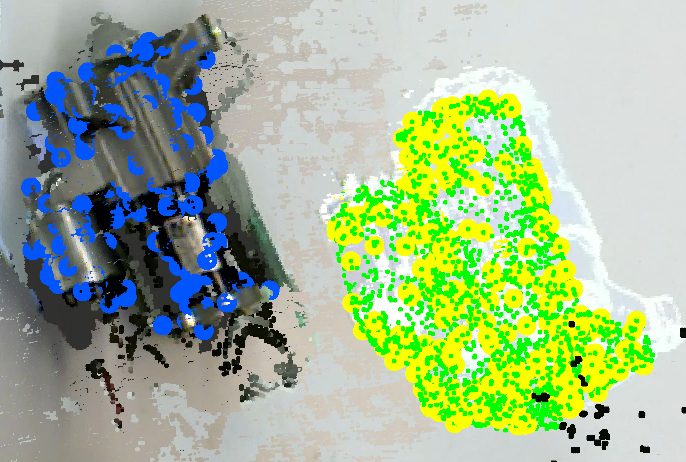
\includegraphics[height=.27\textheight]{initial-pose-estimation-1-before}
	\hspace{0.5em}
	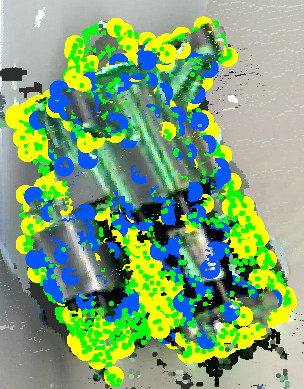
\includegraphics[height=.27\textheight]{initial-pose-estimation-1-after}
	\caption{Initial pose estimation of assembled object}
\end{figure}

\begin{figure}[!ht]
	\centering
	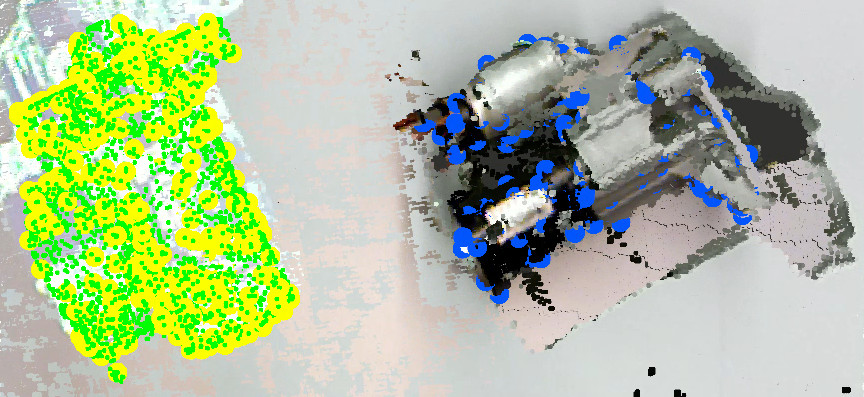
\includegraphics[height=.182\textheight]{initial-pose-estimation-2-before}
	\hspace{0.5em}
	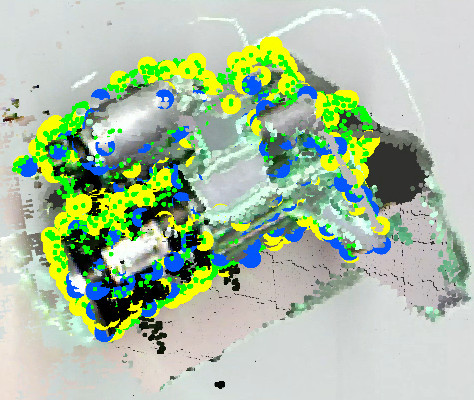
\includegraphics[height=.182\textheight]{initial-pose-estimation-2-after}
	\caption{Initial pose estimation of assembled object}
\end{figure}
